\documentclass[10pt, a4paper, twocolumn]{jarticle}
%\documentclass[10pt, a4paper, twocolumn, uplatex]{jsarticle}
\usepackage{proceeding_bachelor}
\usepackage{tabularx}
\usepackage{booktabs}
\usepackage{multirow}
\usepackage{cite}
\usepackage{amsmath, amssymb}
\usepackage{svg}

% Title info. ======================================
\title{不確実性適応型損失関数による \\
頑健な医用画像セグメンテーション}

%%%%% 著者 %%%%%
\author{廣池 友哉}

%%%% 学籍番号 %%%%
\studentid{M243422}

%%%% 所属 %%%%
\affiliation{広島大学 大学院先進理工系科学研究科 情報科学プログラム}

%%%% 年度を書き換える %%%%
\proceedingname{2025年度修士論文中間発表予稿}

%%%% 卒論発表の日付を書く %%%%
\date{2025/9/19}


\begin{document}
%%%%%%%%%%%%% Header and Title %%%%%%%%%%%%%
\maketitle


%%% Please write your body text from here %%
\section{はじめに}
医用画像セグメンテーションは,医用画像中の全てのピクセルに対し
物体のクラスのラベルを推定することで,正常組織または異常組織の領域を抽出するタスクである.
特に近年では,ポリープ\cite{ji2022video}や頭頸部がん(HNC)放射線治療における危険臓器\cite{maleki2020machine}などに用いられている.

医用画像セグメンテーションは,多様な症例に対して頑健に機能することが求められるが,
対象領域のサイズや形状が画像ごとに大きく異なるため,頑健な検出が困難であるという課題がある.
この課題に対処するために,損失関数を工夫する手法が提案されてきた.
例えば分類タスクで広く使われているCross-Entropy Loss\cite{long2015fully}と比較して,
Dice Index と呼ばれる類似度指標に基づいて定義されているDice Loss\cite{milletari2016v}は,
少数クラスの誤差も全体の平均損失に大きく寄与するため,クラス不均衡下でも検出性能を向上させる効果がある.
また、Dice Lossの多くの拡張手法も提案されており,CT画像\cite{zhu2019anatomynet, 9109297}や
MRI画像\cite{KATO2024107695}において高い性能が報告されている.
しかし,これらのアプローチでは検出難易度に関わらず誤差関数の形状が固定されており,
検出難易度が高い画像に対する学習が不十分になり,頑健な検出が困難であるという課題がある.

そこで本研究では,検出難易度を画像毎に算出したものを学習に取り入れ,
誤差関数の形状を動的に変化させる手法を提案する.
具体的には,画像毎に形状を変更できる誤差関数であるPolyDice-1 Lossを用いる.
学習中には一定epoch毎に推論フェーズを挿入し,Monte Carlo Dropout\cite{pmlr-v48-gal16}(以下,MC Dropout)により
各画像毎に複数枚の予測画像を得た後,ピクセル単位で不確実性指標を計算し,そこから画像全体の不確実性指標を集約したものを難易度指標として算出する.
この難易度指標をPolyDice-1 Lossの学習に取り入れることで,検出難易度を考慮した頑健な検出を実現することができる.

\section{提案法}

\subsection{概要}
本研究の最終目標は,画像ごとのセグメンテーション難易度を学習中に動的に評価し,
その難易度に応じて損失関数の形状を適応的に変化させるシステムの構築である.
図に提案法の全体構成を示す.
提案法では,学習中各画像に対してMC Dropoutを用いて画像毎に複数枚推論を行い,予測のばらつきから不確実性を定量化する.
この不確実性情報は,モデルがその画像のセグメンテーションをどの程度「難しい」と感じているかを反映する.
将来的には,この不確実性情報を画像単位に集約し,PolyDice-1 Lossのハイパーパラメータ$\epsilon$を動的に制御することで,
難しい画像には急峻な勾配を,簡単な画像には緩やかな勾配を与える適応的学習を実現する.

本稿では,最終目標に向けた基礎的検証として,ピクセル単位の不確実性指標が学習過程でどのように推移するかを分析し,
画像難易度の指標としての妥当性を検証する.

\subsection{PolyDice Lossによる損失形状制御}

\subsubsection{Dice Lossの定式化}
画像サイズを $H \times W$とし,ピクセル位置を $(i, j)$ で表す($i \in \{1, ..., H\}, j \in \{1, ..., W\}$).
セグメンテーションタスクにおいて,モデルの予測確率マップを$\hat{\mathbf{y}} \in \mathbb R ^ {H \times W}$,
その画像に対する正解マスクを$\mathbf{y} \in \mathbb R ^ {H \times W}$とすると,Dice Lossは次式で定義される.

\begin{equation}
  \mathcal{L}_{\text{Dice}}(\hat{\mathbf{y}}, \mathbf{y}) = 1 - \frac{2 \sum_{i=1}^{W} \sum_{j=1}^{H} \hat{y}_{ij} y_{ij}}{\sum_{i=1}^{W} \sum_{j=1}^{H}(\hat{y_{ij}} ^ 2 + y_{ij} ^ 2)}
\end{equation}

\subsubsection{幾何学的解釈と多項式展開}

予測確率マップ$\hat{\mathbf{y}}$と正解マスク$\mathbf{y}$をそれぞれ長さ$HW$のベクトル$\hat{\mathbf{y}} ^ {\prime}, {\mathbf{y}} ^ {\prime}$
として平坦化すると,Dice Lossは以下のように分解できる.

\begin{equation}
  \mathcal{L}_{\text{Dice}} = 1 - s \cos  \theta
\end{equation}
% \begin{equation}
%   \begin{aligned}
%     \mathcal{L}_{\text{Dice}} &= 1 - \frac{2 \langle \hat{\mathbf{y}} ^ {\prime}, {\mathbf{y}} ^ {\prime} \rangle}{\Vert \hat{\mathbf{y}} ^ {\prime} \Vert ^ 2 + \Vert {\mathbf{y}} ^ {\prime} \Vert ^ 2} \\
%     &= 1 - \frac{2 \Vert \hat{\mathbf{y}} ^ {\prime} \Vert \Vert {\mathbf{y}} ^ {\prime} \Vert}{\Vert \hat{\mathbf{y}} ^ {\prime} \Vert ^ 2 + \Vert {\mathbf{y}} ^ {\prime} \Vert ^ 2}
%     \times \frac{\langle \hat{\mathbf{y}} ^ {\prime}, {\mathbf{y}} ^ {\prime} \rangle}{\Vert \hat{\mathbf{y}} ^ {\prime} \Vert \Vert {\mathbf{y}} ^ {\prime} \Vert}
%   \end{aligned}
% \end{equation}
ここで,$s = \frac{2 \langle \hat{\mathbf{y}} ^ {\prime}, {\mathbf{y}} ^ {\prime} \rangle}{\Vert \hat{\mathbf{y}} ^ {\prime} \Vert ^ 2 + \Vert {\mathbf{y}} ^ {\prime} \Vert ^ 2}$はスケール成分,
$\theta = \frac{\langle \hat{\mathbf{y}} ^ {\prime}, {\mathbf{y}} ^ {\prime} \rangle}{\Vert \hat{\mathbf{y}} ^ {\prime} \Vert \Vert {\mathbf{y}} ^ {\prime} \Vert}$は2つの
ベクトル間の角度を表す.この分解により,Dice Lossはスケール成分$s$と$\cos \theta$の積として理解できる.

方向成分$\cos \theta$に対してTaylor展開を適用することで,PolyDice Lossの多項式表現を導出する.
つまり$\theta \approx 0$(予測と正解が大きく異ならない)と仮定し,$\cos{\theta}$を$\theta = 0$まわりでテイラー展開すると以下のように近似できる.
\begin{equation}
  \cos{\theta} = 1 - \frac{\theta ^ 2}{2!} + \frac{\theta ^ 4}{4!} - \cdots
\end{equation}
これをDice Lossに代入し,整理するとPolyDiceの一般形が得られる:
% \begin{equation}
%   \begin{aligned}
%   \mathcal{L}_{\text{Dice}} &= 1 - s \left(1 + \frac{1}{2!} \theta ^ 2 - \frac{1}{4!} \theta ^ 4 + \cdots\right) \\
%   &= (1 - s) + s \left[\sum_{k = 1}^{\infty} \frac{(-1) ^ {k - 1}}{(2k)!} \theta ^ {2k}\right]
% \end{aligned}
% \end{equation}
\begin{equation}
  \mathcal{L}_{\text{PolyDice}} = (1 - s) + s \sum_{k = 1}^{\infty} \alpha_k \theta ^ {2k}
\end{equation}
ここで, $\alpha_k=\frac{(-1)^{k-1}}{(2k)!}$は各Taylor項の符号係数である.

% この損失関数を計算するために、角度$\theta$は以下のようにコサインの逆関数を用いて算出される.
% \begin{equation}
%   \theta = \arccos{\left(\frac{\langle \hat{\mathbf{y}} ^ {\prime}, {\mathbf{y}} ^ {\prime} \rangle}{\Vert \hat{\mathbf{y}} ^ {\prime} \Vert \Vert {\mathbf{y}} ^ {\prime} \Vert}\right)}
% \end{equation}

\subsubsection{PolyDice-1 Loss}
実用的な観点から,\cite{leng2022polyloss}のアプローチに従い,第$1$項のみを調整可能とするPolyDice-1 Lossを採用する:
\begin{equation}
  \mathcal{L}_{\text{PolyDice-1}} = (1 - s) + s \left(\frac{1}{2} + \epsilon\right) \theta^2
\end{equation}
ここで,$\epsilon \in \mathbb{R}$は損失関数の形状を制御する唯一のハイパーパラメータである.
図\ref{polydice}に$s = 0.1$としてPolyDice-1 Lossの$\epsilon$を変化させた際の値の推移を示す.
$\epsilon > 0$では予測誤差に対するペナルティが強化され,$\epsilon < 0$では緩和される.
本稿では,まず$\epsilon = 0$で固定して実験を行い,将来的にはこの$\epsilon$を不確実性に基づいて動的に調整する.

\begin{figure}
  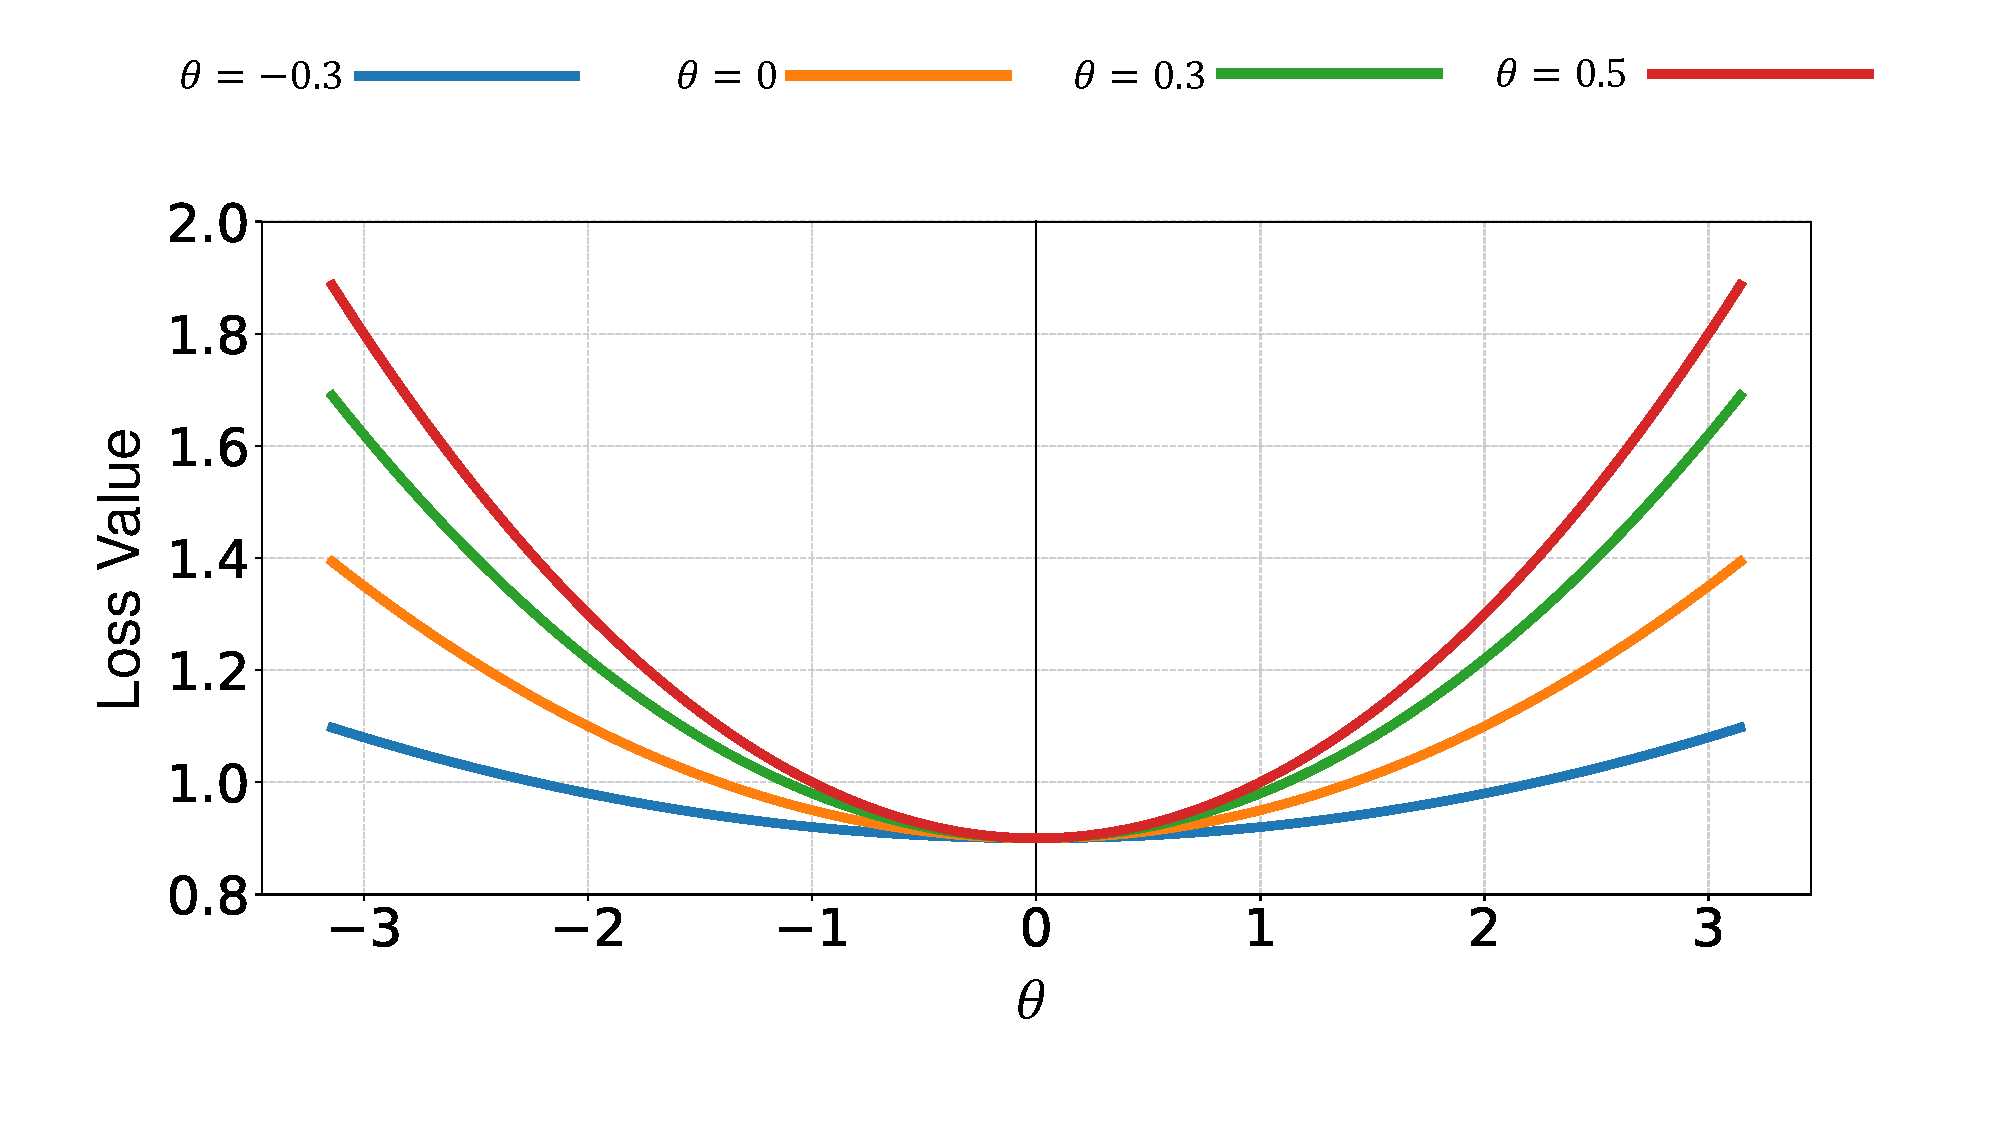
\includegraphics[scale=0.25]{figure/loss.pdf}
  \caption{Plot of PolyDice-1 Loss($s = 0.1$)}
  \label{polydice}
\end{figure}

\subsection{MC Dropoutによる不確実性推定}

\subsubsection{MC Dropoutの理論的背景}

Dropoutは,ニューラルネットワークの学習時に,一部のユニットを確率$p$でランダムに不活性化することで
過学習を抑制し,モデルの汎化性能を向上させる手法である.

MC Dropoutは.学習時のみだけでなく.推論時にもDropoutを用いることで不確実性を推定する手法である.
通常,推論時の出力は決定論的であるが,Dropoutを有効にすることで,
異なるサブネットワークが形成され、確率的な出力が得られる.
同一入力に対してこの確率的な推論を複数回実行して得られる予測結果の分布は、
Bayesian Neural Networkにおける予測事後分布近似とみなせ,変分推論の一種として解釈できる.
提案法では,学習段階でM(epoch)毎に推論フェーズを挿入してDropoutを確率$p$でMC Dropoutを$N$回実行することで,
各学習段階で$N$枚の複数の予測画像を得る.
またDropout層はモデルの最も深いエンコーダおよびデコーダに配置する.
浅い層と比較してより高次な特徴を抽出する深い層でDropoutを実行することで,
高次な意味的判断におけるモデルの確信度がより直接的に反映されることが期待される.

\subsubsection{MC Dropoutの定式化}
学習済みモデル$f_{\theta}: \mathcal{X} \rightarrow [0,1]^{H \times W}$に対し,Dropout率$p \in (0,1)$でMC Dropoutを適用する.
同一入力画像$x \in \mathcal{X}$に対してN回の確率的推論を行い,予測集合$\{\hat{Y}^{(n)}\}_{n=1}^{N}$を得る:
%
\begin{equation}
  \hat{Y}^{(n)} = f_{\theta}(x; \mathbf{z}^{(n)}), \quad \mathbf{z}^{(n)} \sim \text{Bernoulli}(1-p)
\end{equation}
%
ここで,$\mathbf{z}^{(n)}$は$n$回目の推論におけるDropoutマスク(各ニューロンの活性/非活性を決定)である.
各$\hat{Y}^{(n)} = \{\hat{y}_{i,j}^{(n)} \in [0,1]\}_{i,j}$は$n$回目の推論における予測確率マップである.

\subsubsection{ピクセル単位の不確実性指標の計算}
得られた$N$枚の予測画像に対し,ピクセル単位で不確実性指標を計算する.
不確実性マップから,以下の3つの不確実指標をピクセル単位で計算する.

\begin{itemize}
  \item \textbf{予測分散}:
  \begin{equation}
    \text{Var}(\hat{y}_{ij}) = \frac{1}{N} \sum_{n=1}^{N} (\hat{y}_{ij}^{(n)} - \bar{y}_{i,j})^2
  \end{equation}
  ここで,$\bar{y}_{i,j} = \frac{1}{N} \sum_{k = 1}^{N} \hat{y}_{ij} ^ {(n)}$は予測の平均である.
  この指標は,複数回の予測がどの程度ばらついているかを表し,値が大きいほどモデルの予測が不安定であることを示す.
  \item \textbf{予測エントロピー}:
  \begin{equation}
    H(\bar{y}_{i,j}) = - \mu_{ij} \log{\bar{y}_{i,j}} - (1 - \bar{y}_{i,j}) \log{(1 - \bar{y}_{i,j})}
  \end{equation}
  これは平均予測の不確実性を表す.エントロピーは予測確率が$0.5$に近いほど高くなり,
  モデルが前景・背景の判断に迷っていることを示す.確率が$0$または$1$に近い場合は低い値となる.
  \item \textbf{相互情報量}:
  \begin{equation}
    I(\hat{y}_{ij}) = H(\bar{\hat{y}}_{ij}) - \frac{1}{N}\sum_{n=1}^{N} H(\hat{y}_{ij}^{(n)})
  \end{equation}
  これはモデルパラメータの不確実性(認識的不確実性)を表す.
  全体の不確実性から偶然的不確実性を引いたもので,より多くのデータで学習することで減少する性質を持つ.
  この値が高い領域は,モデルが十分に学習できていない可能性を示唆する.
\end{itemize}

\subsection{画像全体の難易度への集約と適応的制御(将来構想)}

\subsubsection{画像単位への集約}
ピクセル単位の不確実性マップ$U = \{u_{i,j}\}_{i,j}$から画像全体の難易度スコア$D \in \mathbb{R}^+$を算出する必要がある.
セグメンテーションタスクの特性を考慮すると,境界領域の不確実性に着目する方法や,予測誤差と相関の高い領域を重視する方法などが考えられる.
また,不確実性の空間的分布パターンや,前景・背景それぞれの不確実性の違いも重要な情報となる可能性がある.

\subsubsection{適応的パラメータ制御}
画像難易度スコア$D$に基づいて,Poly Dice Lossのパラメータ$\epsilon$を動的に制御する:

\begin{equation}
  \epsilon = g(D; \theta_g)
\end{equation}
ここで,$g$は制御関数,$\theta_g$はその学習可能なパラメータである.
難易度が高い画像には大きな$\epsilon$を割り当てて急峻な勾配を与え,
簡単な画像には小さな$\epsilon$で緩やかな勾配を与えることで,効率的な学習を実現する.


\newpage

\section{実験}
\subsection{実験設定}
\subsubsection{データセット}
画像難易度の指標としての妥当性を検証するために,医用画像セグメンテーションデータを用いて実験を行った.
データセットは,$384 \times 288$ pixelの$612$枚の大腸内視鏡画像とポリープマスクが含まれるCVC-ClinicDB\cite{BERNAL201599}を用い,
訓練データとテストデータの割合は$8:2$とし,訓練データのうち$10 \%$をランダムに抽出し,検証データとした.

\subsubsection{実装の詳細}
セグメンテーションモデルは$3$層のU-Net\cite{ronneberger2015u}を用い,
学習には,バッチサイズ$32$, 学習率$10 ^ {-3}$ のAdaptive moment
estimation(以下, Adam)\cite{kingma2014adam}を用いた.
損失関数はPolyDice-1 Lossにおいて$\epsilon = 0$としたものを用いた.
各画像は$W = 224$ pixel, $H = 224$ pixelでリサイズを行い,
過学習抑制のため,訓練データに対する空間的データ拡張として
$50\%$の確率で上下左右反転及び画像の明るさ・コントラストの変更を施した.
最大エポック数は$200$に設定し,検証データに対する損失が最小のエポックにおける
モデルインスタンスを,最終的なテストデータの評価に用いた.
また,提案法におけるMC Dropoutのパラメータとして,
Dropoutを行う確率$p = 0.5$,推論回数$N = 10$,推論フェーズの挿入間隔$M = 10$とした.

\subsection{結果と考察}

\subsubsection{学習過程における不確実性の推移}
学習初期に高い精度で予測できるようになった症例(以下症例$1$)と,学習後期においても精度が低い症例(以下症例$2$)について,
$50, 100, 150, 200$ epochのピクセル単位の不確実性指標の推移を示す.
(a)は予測平均,(b)は予測分散,(c)は予測エントロピー,(d)は相互情報量である.
なお各不確実性指標において,カラースケールは両症例間で統一し,全ピクセル・全エポックにおける最大値で正規化した.

図\ref{fold5_file144}に症例$1$の不確実性指標の推移を示す.
図\ref{fold5_file144}(b),(d)から,学習の進行に伴いポリープ内外で減少していることがわかる.
一方,両指標ともにポリープの境界部分では,学習後期においても微小な不確実性が残存している.

図\ref{fold2_file450}に症例2の不確実性指標の推移を示す.
図\ref{fold2_file450}(b),(d)から,症例$1$と異なり,学習の進行に伴い,
ポリープの輪郭および内部において不確実性が増大していることがわかる.

今回の検証から,各不確実性指標が捉える「難しさ」の側面が明らかになった.
学習に伴い,相互情報量は症例1では減少し,症例2では増大したことから,
これらはモデルの知識不足に起因するエピステミック不確実性を主に捉える指標と言える.
一方,予測エントロピーは,学習が十分に進んで病変の特徴を捉えた後でも,画像の境界領域で高い値を示した.
これは,「データ固有の曖昧さ」に起因するアレアトリック不確実性を捉える指標と言える.

検証の結果,学習の進行に伴い,高精度な症例では相互情報量が収束したのに対し,
精度が低い症例では学習後期でも高い相互情報量が残存することが確認された.
本研究の目的は,損失関数を動的に制御して精度を向上させることにあるため,改善の余地がある「モデルの知識不足」を特定することが重要となる.
したがって,モデルが「迷っている」状態を最も直接的に示す相互情報量が,本研究における難易度指標として妥当であると考えられる.
検証の結果から,集約された難易度指標の値が高く難しい画像にはPolyDice-1 Lossの係数$\epsilon$を増加させ,
急峻な勾配を課す適応的な学習を行うことで,特徴を重点的に学習させることができると考えられる.
本稿の分析で,困難な症例では不確実性がポリープの内部に広範囲に分布する傾向が確認された.
この情報をより効果的に活用するため,病変の正解マスクに着目して相互情報量を集約することで,
難しい症例に対して頑健な検出ができる指標の設計を目指す.

\section{まとめと今後の課題}
本稿では,医用画像セグメンテーションの誤差関数において,検出難易度が高い画像に対する学習が不十分になり,頑健な検出が困難であるという課題に対処するため,
検出難易度を画像毎に算出したものを学習に取り入れ,誤差関数の形状を動的に変化させる手法を提案した.
提案法では,学習中各画像に対してMC Dropoutを用いて画像毎に複数枚推論を行い,
予測のばらつきから不確実性を定量化した.
医用画像データセットを用いた実験の結果,学習後期においても精度が低い症例に関して,
ピクセル単位の相互情報量の分散と相互情報量が増大していくことが明らかになった.
今後は,上記の不確実性指標を領域周辺に着目して集約する方法を検討し,
難易度が高い画像には急峻な勾配を与えることで,精度が低い症例でも頑健な検出を実現できる
制御関数を実装し,提案法の有効性を検証する予定である.
\newpage

\begin{figure*}[t] % ← [t]をここに移動する
  \begin{center}
    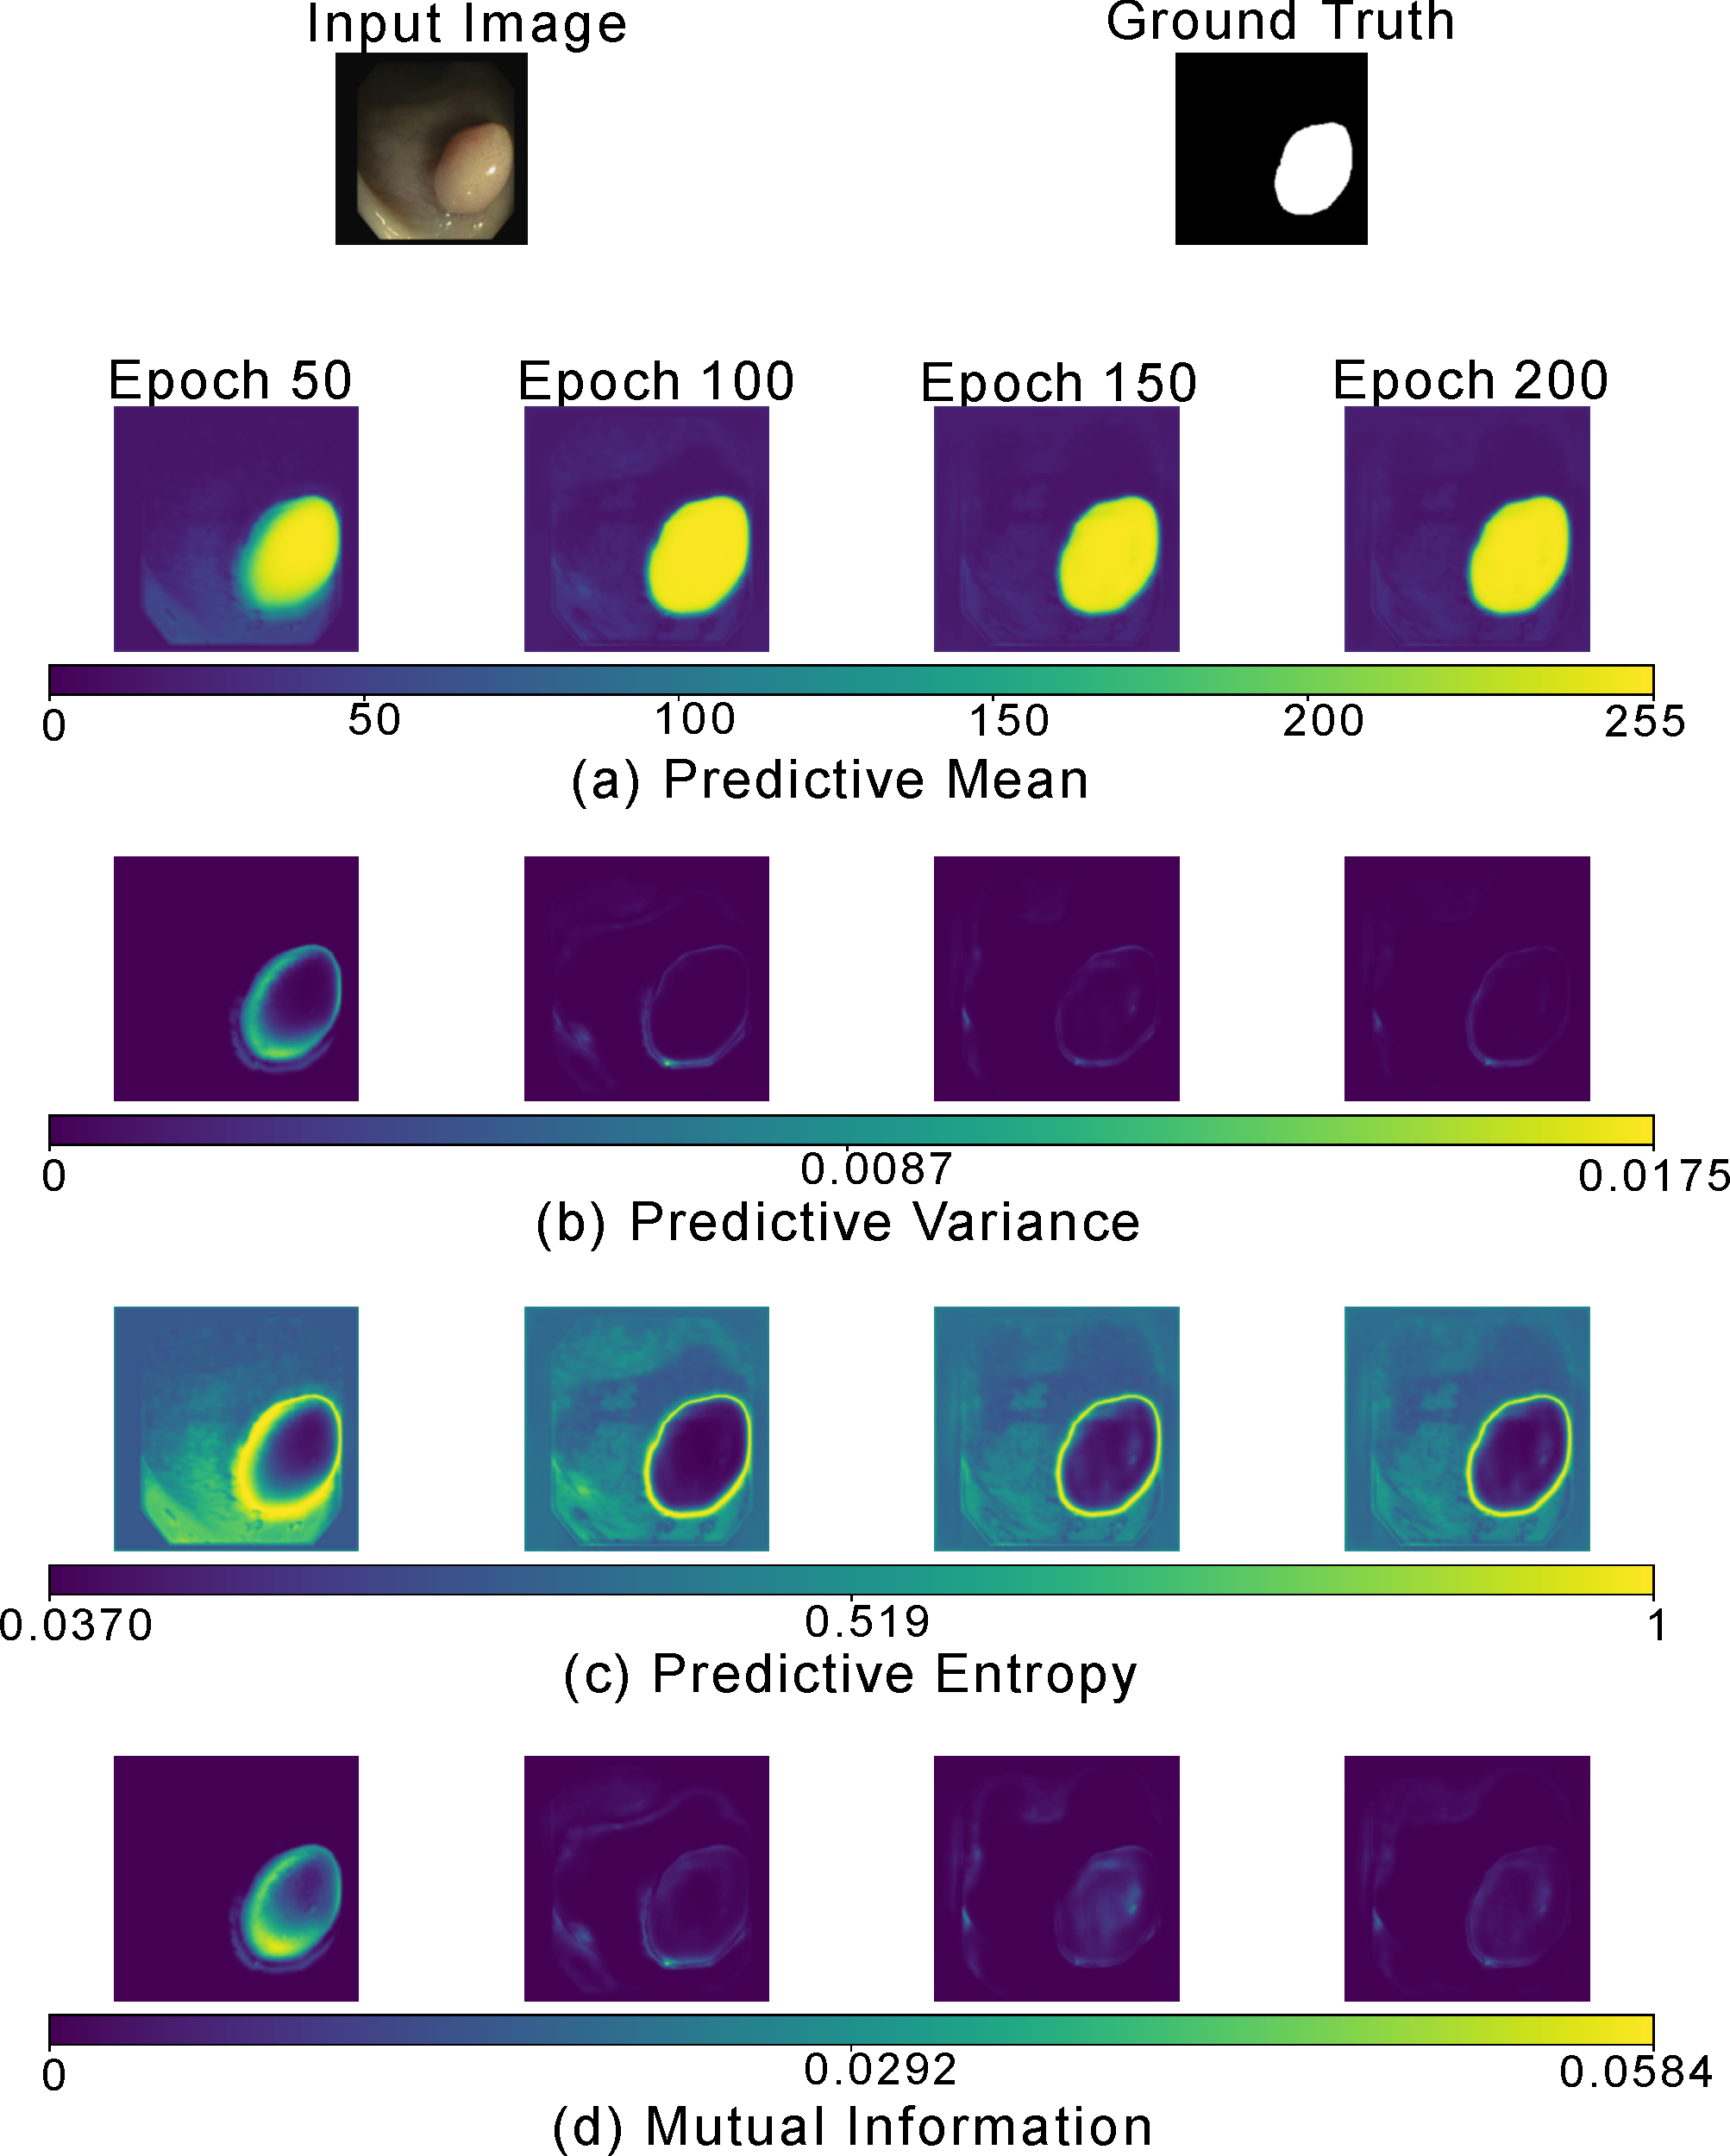
\includegraphics[scale=0.25]{figure/fold5_file144_uncertainty_evolution.pdf}
    \caption{Example of Cases that are learned quickly with high accuracy:
    (a) Predictive Mean, (b) Predictive Variance,
    (c) Predictive Entropy(d) Mutual Information}
    \label{fold5_file144}
  \end{center}
\end{figure*}

\begin{figure*}[t] % ← [t]をここに移動する
  \begin{center}
    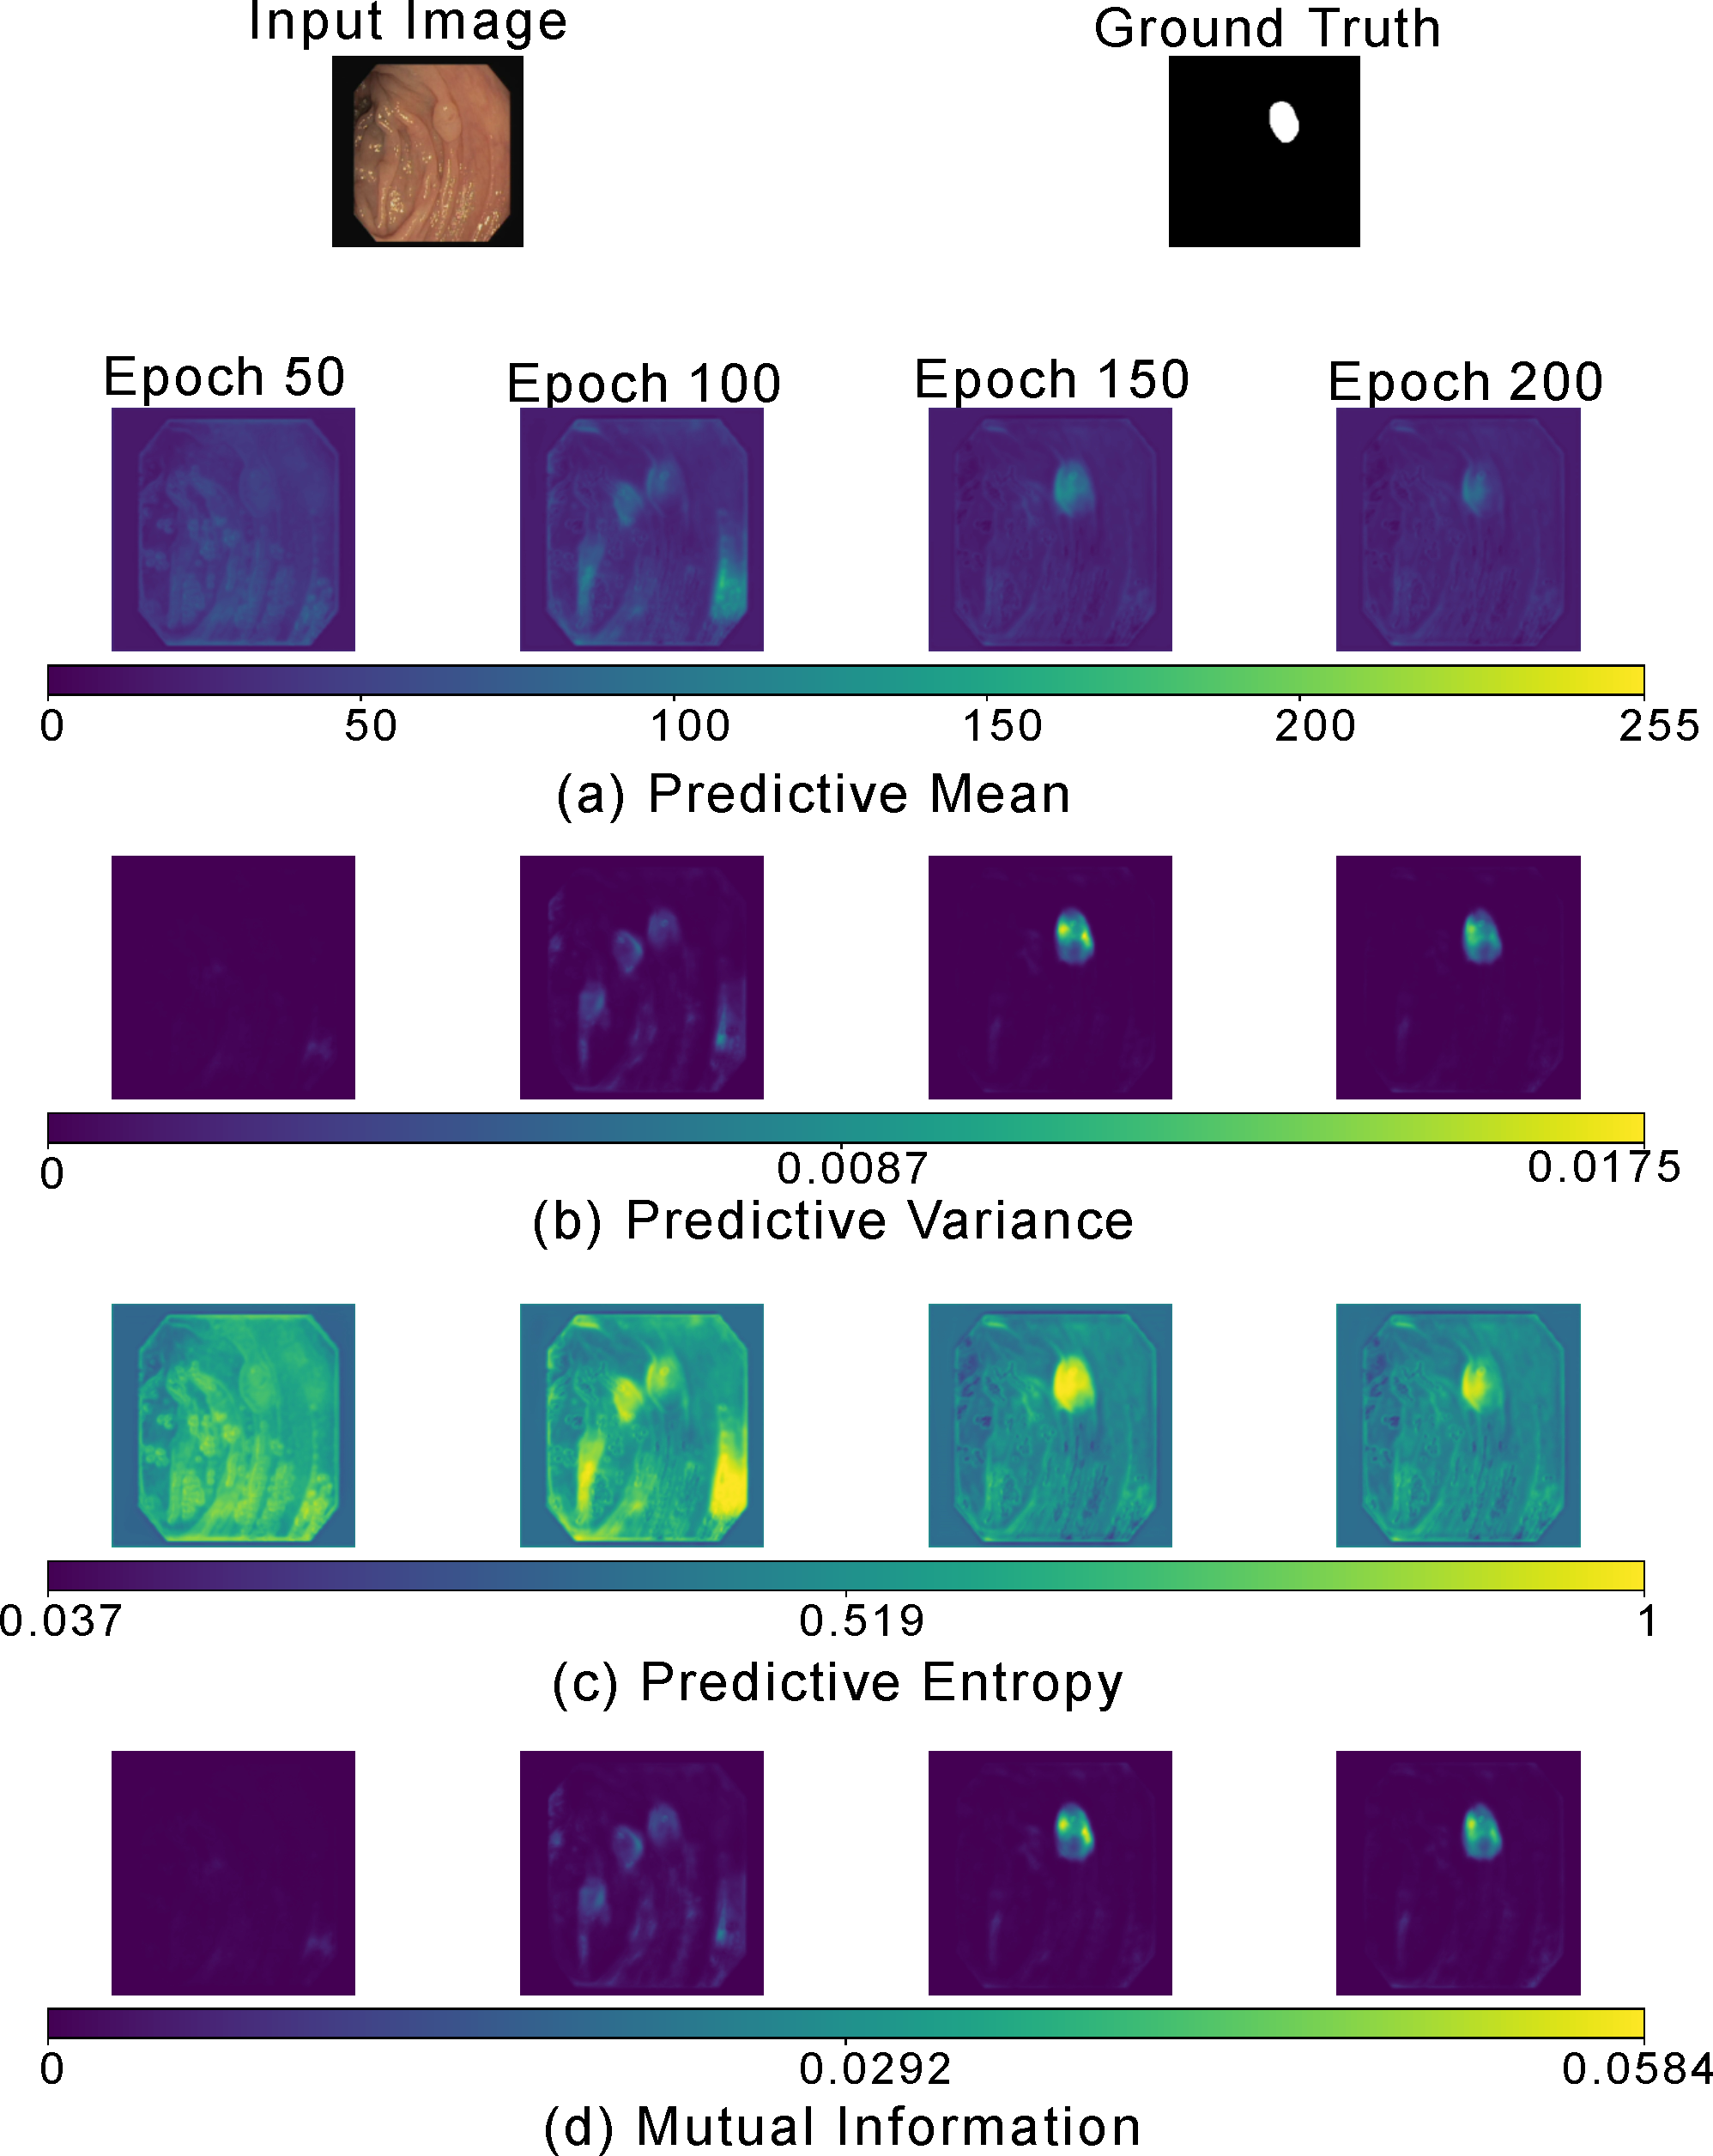
\includegraphics[scale=0.25]{figure/fold2_file450_uncertainty_evolution.pdf}
    \caption{Example of Challenging cases with persistently low performance:
    (a) Predictive Mean, (b) Predictive Variance,
    (c) Predictive Entropy(d) Mutual Information}
    \label{fold2_file450}
  \end{center}
\end{figure*}

\clearpage

%%%%% 参考文献(BibTeXを使う場合) %%%%%
\bibliographystyle{bibstyle} % bstファイルを設定
\bibliography{references} % bibファイルを読み込み

%%%%% 参考文献(直接書く場合) %%%%%
% \begin{thebibliography}{9} %\footnotesize
    % \bibitem{kajiya1986rendering}
    % J.~T. Kajiya,
    % \newblock ``The rendering equation,''
    % \newblock in {\em Proceedings of the 13th Annual Conference on Computer
    %   Graphics and Interactive Techniques}, pp. 143--150, 1986.
    
    % \bibitem{jensen2001realistic}
    % H.~W. Jensen,
    % \newblock {\em Realistic image synthesis using photon mapping}, vol. 364,
    % \newblock Ak Peters Natick, 2001.
% \end{thebibliography}

\end{document}